\documentclass{article}

\usepackage{geometry}
\usepackage{amsmath}
\usepackage{graphicx}
\usepackage{listings}
\usepackage{hyperref}
\usepackage{multicol}
\usepackage{fancyhdr}
\pagestyle{fancy}
\hypersetup{ colorlinks=true, linkcolor=black, filecolor=magenta, urlcolor=cyan}
\geometry{ a4paper, total={170mm,257mm}, top=20mm, right=20mm, bottom=20mm, left=20mm}
\setlength{\parindent}{0pt}
\setlength{\parskip}{1em}
\renewcommand{\headrulewidth}{0pt}
\lhead{Competitive Programming - Arkavidia V}
\fancyfoot[CE,CO]{\thepage}

\begin{document}

\begin{center}
    \section*{D. DVD} % ganti judul soal

    \begin{tabular}{ | c c | }
        \hline
        Batas Waktu  & 1s \\    % jangan lupa ganti time limit
        Batas Memori & 64MB \\  % jangan lupa ganti memory limit
        \hline
    \end{tabular}
\end{center}

\subsection*{Deskripsi}

\begin{center}
    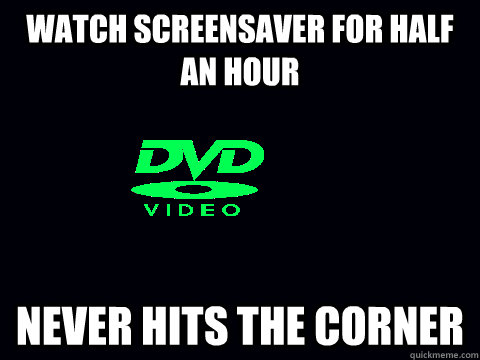
\includegraphics[width=200px]{meme}
\end{center}

\begin{multicols}{2}

Arvy sedang memandang monitornya yang berukuran $W \times H$ satuan.
Di monitornya, sedang berjalan \textit{screen saver} DVD.
Pada \textit{screen saver} ini, logo DVD bergerak lurus.
Ketika menyentuh sisi monitor, logo DVD akan berubah warna dan memantul dengan sudut datang sama dengan sudut pantul (perhatikan gambar di samping).

\begin{center}
    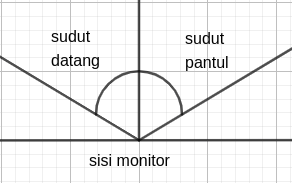
\includegraphics[width=140px]{pantul}
\end{center}
\end{multicols}

Arvy lelah menonton \textit{screen saver} DVD yang terus memantul-mantul.
Ia menunggu kapan logo DVD menyentuh di sudut monitor.
Ia mulai ragu apakah logo DVD akan menyentuh di sudut monitor.
Ia memiliki koordinat lokasi DVD sekarang (monitor digambarkan sebagai persegi panjang di koordinat kartesian dengan titik $(0, 0)$ di kiri bawah dan $(W, H)$ di kanan atas) dan vektor arah gerak logo yang dideskripsikan sebagai $(v_x, v_y)$ (Anda dapat menganggap logo sebagai sebuah persegi panjang dengan ukuran lebar $w_l$ dan tinggi $h_l$).
Tentukan apakah logo akan menyentuh sudut monitor (salah satu ujung persegi panjang logo berhimpit dengan sudut monitor)!

\subsection*{Format Masukan}

Baris pertama terdiri dari satu bilangan bulat positif $T$ ($1 \leq T \leq 1.000$), menyatakan banyaknya kasus uji.

Untuk tiap kasus uji, akan terdapat 2 baris.
Baris pertama terdiri dari $W$, $H$ ($3 \leq W, H \leq 1.000.000.000$), menyatakan ukuran monitor dan $w_l$ ($1 \leq w_l \leq W$), $h_l$ ($1 \leq h_l \leq H$) menyatakan ukuran logo DVD.
Baris kedua terdiri dari $x$ ($0 \leq x \leq W - w_l$), $y$ ($0 \leq y \leq H - h_l$) menyatakan letak titik kiri bawah logo sekarang dan $v_x, v_y$ ($-1.000.000.000 \leq v_x, v_y \leq 1.000.000.000$) menyatakan vektor arah gerak logo.

\subsection*{Format Keluaran}

Untuk tiap kasus uji, tuliskan \lstinline{YA} jika logo DVD akan menyentuh koordinat tepat sudut monitor, atau \lstinline{TIDAK} jika tidak.
\\

\begin{multicols}{2}
\subsection*{Contoh Masukan}
\begin{lstlisting}
3
7 8 2 3
1 2 4 4
7 4 1 1
3 3 1 -1
9 9 3 4
6 3 -3 -1
\end{lstlisting}
\columnbreak
\subsection*{Contoh Keluaran}
\begin{lstlisting}
TIDAK
YA
YA
\end{lstlisting}
\vfill
\null
\end{multicols}

\subsection*{Penjelasan}
Untuk kasus uji pertama, monitor dapat digambarkan seperti persegi panjang $ABCD$ di bawah, dengan pergerakan logo DVD digambarkan seperti persegi panjang $EFGH$

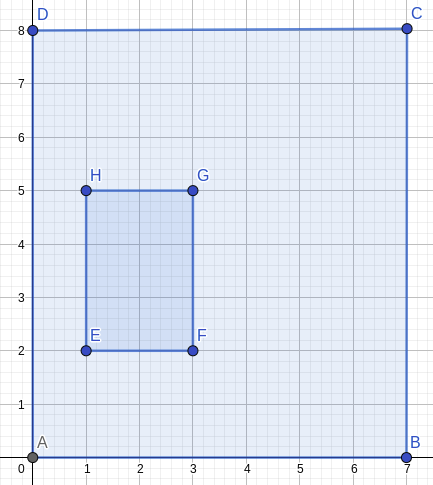
\includegraphics[width=80px]{sample-1-1}
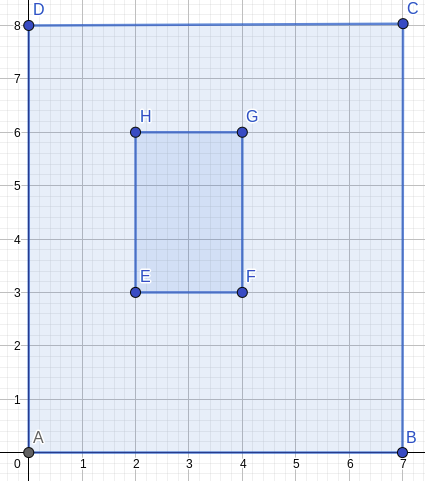
\includegraphics[width=80px]{sample-1-2}
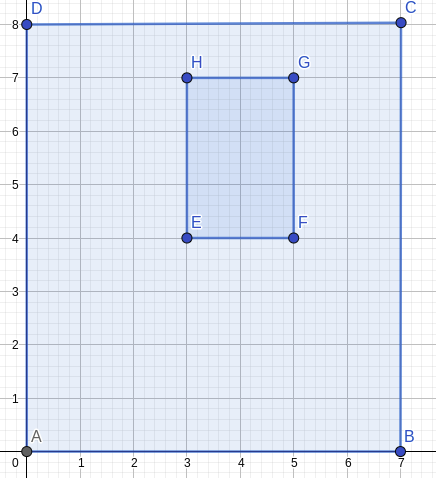
\includegraphics[width=80px]{sample-1-3}
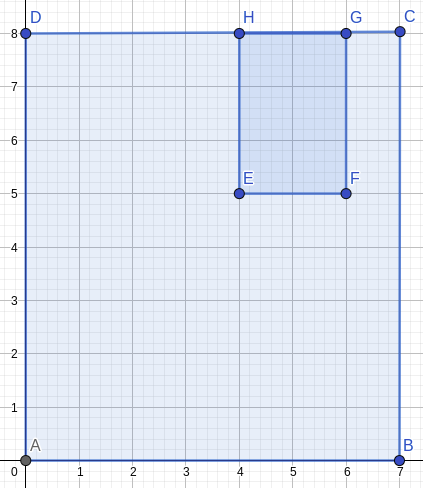
\includegraphics[width=80px]{sample-1-4}
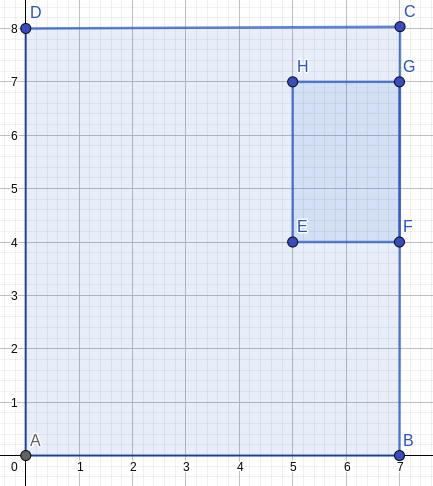
\includegraphics[width=80px]{sample-1-5}
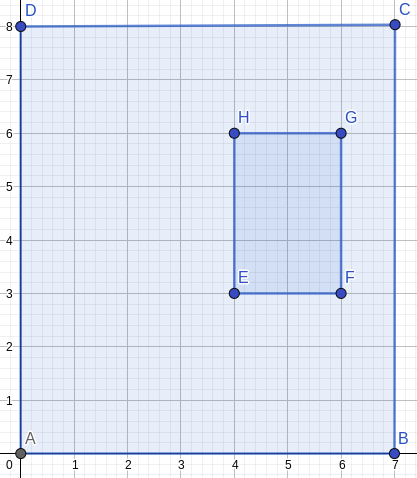
\includegraphics[width=80px]{sample-1-6}

Untuk kasus uji kedua, pergerakan logo DVD akan seperti berikut.

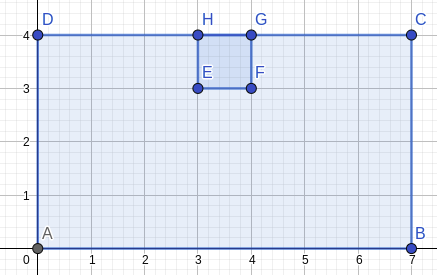
\includegraphics[width=120px]{sample-2-1}
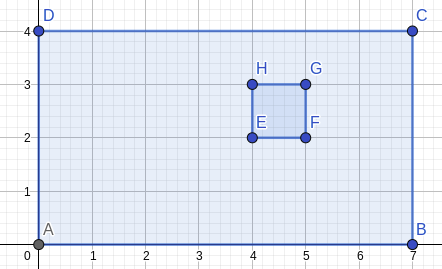
\includegraphics[width=120px]{sample-2-2}
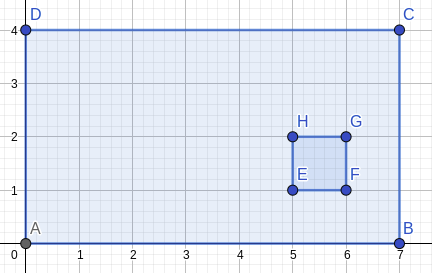
\includegraphics[width=120px]{sample-2-3}
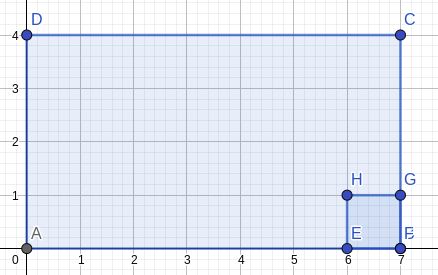
\includegraphics[width=120px]{sample-2-4}

\pagebreak

\end{document}